% Compilar a .pdf con LaTeX (pdflatex)
% Es necesario instalar Beamer 

\documentclass{beamer}

\usepackage{moreverb} 
\usepackage{listings}
\usepackage{mflogo}

% imprimir
% \documentclass[handout]{beamer} 
% \usepackage{pgfpages}
% \pgfpagesuselayout{4 on 1}[a4paper,landscape,border shrink=5mm]

\mode<presentation> {
  %\usetheme{Warsaw}
  \usetheme{Darmstadt}
  \setbeamercovered{transparent}
}

\usepackage[utf8]{inputenc}
\usepackage{graphics}
%\usepackage{amssymb} % Simbolos matematicos

%% Metadatos del PDF.
\hypersetup{  
  pdftitle={F$\ell$OSS HA cluster for Netnovation's ZCS},
  pdfauthor={Daniel G\'amez},
  pdfcreator={Universidad Rey Juan Carlos (Madrid, Spain)},
  pdfproducer=PDFLaTeX,
  pdfsubject={Master in Free Libre Open Source Sorftware},
}
%%

\defbeamertemplate*{footline}{shadow theme}
{
  \leavevmode
  \hbox{
  \begin{beamercolorbox}[wd=.5\paperwidth,ht=2.5ex,dp=1.125ex,leftskip=.3cm plus1fil,rightskip=.3cm]{author in head/foot}
    \usebeamerfont{author in head/foot}\insertframenumber\,/\,\inserttotalframenumber\hfill
\includegraphics[scale=0.40]{img/cc-by-sa-80x15.png} \hspace{0.1cm}\insertshortauthor 
  \end{beamercolorbox}
  
  \begin{beamercolorbox}[wd=.5\paperwidth,ht=2.5ex,dp=1.125ex,leftskip=.3cm,rightskip=.3cm plus1fil]{title in head/foot}
    \usebeamerfont{title in head/foot}\insertshorttitle
  \end{beamercolorbox}}
  
  \vskip0pt
}

\setbeamertemplate{itemize/enumerate subbody begin}{\vspace{0.2cm}}
\setbeamertemplate{itemize/enumerate subbody end}{\vspace{0.3cm}}


\begin{document}

\title{F$\ell$OSS HA cluster for Netnovation's ZCS}
\subtitle{Master Thesis}

\author[Daniel G\'amez]{
Author - Daniel G\'amez \\
Tutor - Dr. Gregorio Robles}
\date{}

% Background Image
% \setbeamertemplate{background}
% {
%     \tikz\node[opacity=0.1] at (current page.center)
%     {
%       \vbox to \paperheight{\vfil\hbox to \paperwidth{\hfil
\includegraphics[scale=1.2]{HA.png}\hfil}\vfil}
%     };
% }

\frame<1>[label=firstframe]
{

  \begin{center}
    
\includegraphics[width=4cm]{img/logoURJC.jpg}\\
    \large{Master in Free Libre Open Source Software}\\
  \end{center}

  \maketitle

}

\normalsize

\section[Index]{}

\begin{frame}%[allowframebreaks]
  \tableofcontents
\end{frame}

  \section{Problem Statement}

\begin{frame}
\frametitle{Problem Statement}

\begin{itemize}
  \item Business continuity, fault tolerant systems
  
  \vspace{0.2cm}
  
  \item Cloud Computing Services (ZCS)
  
  \vspace{0.2cm}
  
  \item Meet Service Level Agreements (SLAs)
\end{itemize}

\end{frame}
  \section{Justification/Motivation}

\begin{frame}
\frametitle{Justification/Motivation}

\begin{itemize}
  \item Give credit to business models based on F$\ell$OSS \\
  - Netnovation: Product Specialists, Hosting Providers \\
  
\includegraphics[scale=0.1]{img/zimbra.png}
  
  \item Show that private enterprise can be benefited by F$\ell$OSS \\
  
\includegraphics[scale=0.1]{img/multiple-logos.png} \\
  And many other: LDAP, BIND, Postfix, OpenSSL, ClamAV, KVM, OpenVZ, etc.
  
\end{itemize}
\end{frame}
  \section{Overall Objectives}

\begin{frame}%[allowframebreaks]
\frametitle{Overall Objectives}

\begin{itemize}
  \item Frame the F$\ell$OSS business model used by Netnovation
  
  \vspace{0.2cm}
  
  \item Show various current alternatives provided by F$\ell$OSS at enterprise level
  
  \vspace{0.2cm}
  
  \item Adapt the proposed solution to the guidelines established by Netnovation
  
  \vspace{0.2cm}
  
  \item Establish an initial reference point for implementing HA private cloud services offered by Netnovation
\end{itemize}

\end{frame}
  \section{Specific Objectives}

\begin{frame}
\frametitle{Specific Objectives}

\begin{itemize}
  \item Implement a F$\ell$OSS HA cluster for Netnovation's ZCS
  \item Perform tests in a controlled laboratory environment in order to promote it to production
  \item Describe the methodology used for the selection of the solution, as well as the process to be implemented
\end{itemize}

\end{frame}
  \section{Scope}

\begin{frame}%[allowframebreaks]
\frametitle{Scope}

\begin{itemize}
  \item 04
\end{itemize}

\end{frame}  
  \section{Related Technologies}

\begin{frame}%[allowframebreaks]
\frametitle{Related Technologies}

\begin{itemize}
  \item 05
  \item Commercial Enterprise Cluster Software
  \item HA F$\ell$OSS based tools
\end{itemize}

\end{frame}
  \section{Methodology}

\begin{frame}%[allowframebreaks]
\frametitle{Methodology}

\begin{itemize}
  \item 06
\end{itemize}

\end{frame}
  \section{Netnovation's Architecture}

\begin{frame}
  \frametitle{Netnovation's Architecture}

  \begin{table}
  \begin{tabularx}{\textwidth}{>{\setlength\hsize{0.4\hsize}\setlength\linewidth{\hsize}}X>{\setlength\hsize{0.6\hsize}\setlength\linewidth{\hsize}}X}

    \begin{itemize}
      \item Infrastructure
      \vspace{0.2cm}
      \item Network Scheme
      \vspace{0.2cm}
      \item Supporting Software:\\
	- UTM EFW\\
	- ProxmoxVE\\
	- FreeNAS\\
	- Zabbix
    \end{itemize}

    &
    
    \vphantom{Infrastructure}
    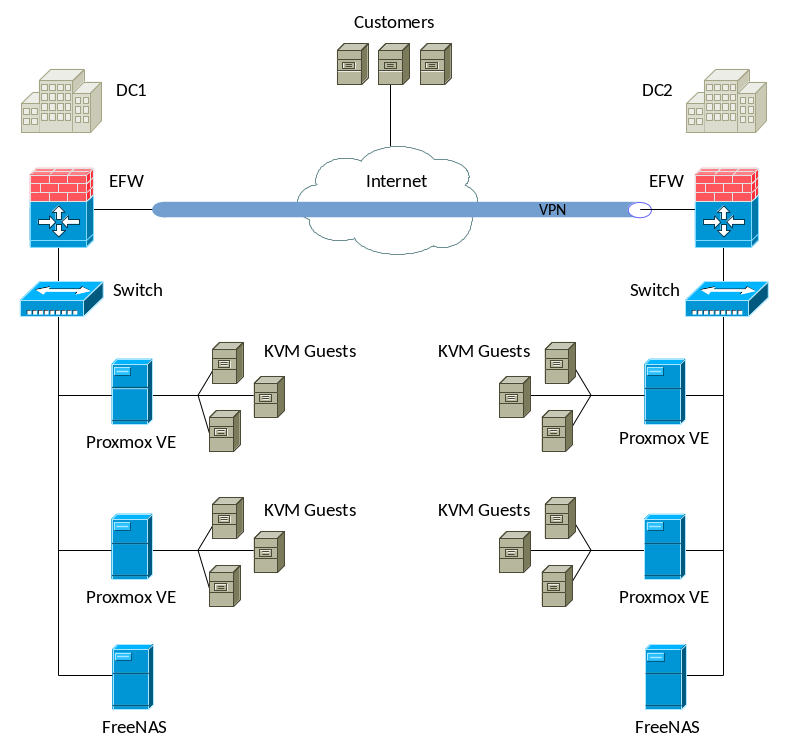
\includegraphics[scale=0.3]{img/network_scheme.png} \\

  \end{tabularx}
  \end{table}

\end{frame}
  \section{Implementation}

\begin{frame}
\frametitle{Implementation}

  \begin{table}
  \begin{tabularx}{\textwidth}{>{\setlength\hsize{0.38\hsize}\setlength\linewidth{\hsize}}X>{\setlength\hsize{0.62\hsize}\setlength\linewidth{\hsize}}X}

    \begin{itemize}
      \item Key software elements
      \vspace{0.2cm}
      \item Technological background
    \end{itemize}
    
    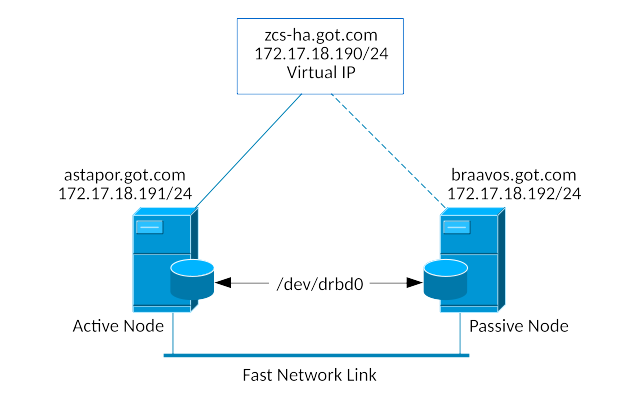
\includegraphics[scale=0.20]{img/two_nodes_ha_cluster.png}

    &
    \vphantom{Key software elements}
    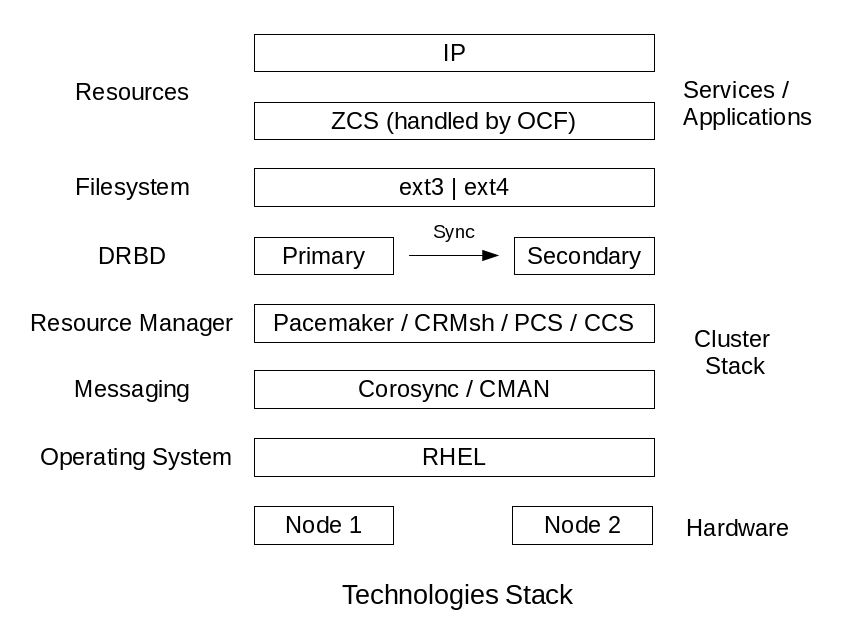
\includegraphics[scale=0.29]{img/implementation-stack.png} \\

  \end{tabularx}
  \end{table}

\end{frame}
  \section{Results}

\begin{frame}
\frametitle{Results}

\begin{itemize}
  \item Research over the Internet, including sources such as FLOSSMetrics
  \item Most of the related projects were currently hosted in GitHub
  \item Since desired solution was enterprise-oriented, focused on a GNU/Linux distribution, main targets were RHEL and SLES
  \item A lot of documentation available for selected technologies (hard to merge)
  \item Metric Grimoire allowed to obtain metrics about selected projects and make some analysis
  \item Methods suggested by Daffara were aptly complemented by LUM
\end{itemize}

\end{frame}
  \section{Conclusions and future work}

\begin{frame}[allowframebreaks]
\frametitle{Conclusions and future work -}

\begin{itemize}
  \item Implications about adopting a cloud infrastructure should be considered (benefits and side effects)
  \item Use of correct technologies directly impact over business continuity
  \item Companies nowadays demand agile decisions at adopting new technologies
  \item Within the significance and contribution of this research are:\\
  - An actual solution for the stated problem has been provided\\
  - Current implementation serves as a reference point for further deployments\\
  - F$\ell$OSS standalone tools are an alternative to enterprise solutions, depending on many factors
  \item For a more comprehensive analysis other tools can be used:\\
  - OpenBRR, QSoS, QualOSS, OSMM
  \vspace{0.2cm}
  \item Other F$\ell$OSS technologies to considerate in order to provide HA for similar environments are:\\
  - OpenStack, Cloudstack, Eucalyptus, OpenNebula, Docker, among many others
  
\end{itemize}

\end{frame}
  \section*{hide}

\begin{frame}%[allowframebreaks]
\frametitle{Bibliography}

\begin{itemize}
  \item 11
\end{itemize}

\end{frame}

\end{document}